% !TeX spellcheck = en_US

\documentclass[a4paper,11pt]{article}
\usepackage{fullpage}
\usepackage[utf8]{inputenc}
\usepackage[T1]{fontenc}
\usepackage{hyperref}
\usepackage{amsmath}
\usepackage{amssymb}
\usepackage{graphicx}
\usepackage{float} % for "H" placement
\usepackage{subcaption} % for subfigures and subtables
\usepackage{booktabs} % enhancement for tables
\usepackage{gensymb} % for \degree
\usepackage{todonotes}

% convenience
\newcommand{\R}{\mathbb{R}}
\DeclareUnicodeCharacter{B0}{\degree}
\DeclareUnicodeCharacter{B1}{$\pm$}


\title{CMLS Homework 1 - Group 9}
%\author{
%	Matteo Bernardini (10743181) \and
%	Francesca Del Gaudio (10768481) \and
%	Valerio Maiolo (10766268) \and
%	Eugenio Poliuti (10724182)
%}
\author{10724182 \and 10743181 \and 10766268 \and 10768481}
\date{}

\begin{document}

	\maketitle
	{\footnotesize\hfill\url{https://github.com/mttbernardini/cmls-hw1}}

	\section{Introduction}

The aim of this document is to describe the realization of a regressor able to predict the mood of a music piece. In particular, in accordance with the Music Emotion Recognition (MER) theory, we used a dimensional approach to face this problem. We considered two ``emotion dimensions'' to describe emotions: the \emph{valence}, that describes the grade of pleasantness, and the \emph{arousal}, which represents the level of intensity of the emotion.

The DEAM Dataset was provided to us. We considered extracts of music pieces, already re-encoded to have the same duration of and the same sampling frequency.
Each annotation related to these songs are provided in terms of mean and standard deviation, for both valence and arousal.
The DEAM Dataset also contains, for each piece, a set of values for already extracted features, as the zero crossing rate, the spectrum centroid, etc. This aspects will be analyzed in detail in section~\ref{sec:database}.

The first step of our research was the \textbf{feature selection}: we studied the usefulness of the provided features, as well as extracting others using the Librosa library in order to have a wider choice. Then, we split the dataset to obtain a training and a testing set. The next step was to implement the \textbf{regressors}, trying with different kinds of them and with different parameters, in order to find the best model. The last step was the \textbf{evaluation} of the prediction, using as metrics the mean squared error and the $R^2$-score.

In the following sections we will analyze in detail our workflow and the tests that led us to our solution of this problem. The document is divided in sections, each one of them describing a different topic we considered for our choices. However they are depending on each other, therefore the flow of this paper does not reflect our chronological approach. Further details can be found in the Jupyter Notebook containing the results of our experiment \cite{notebook} and in the GitHub repository of this assignment \cite{github}.

 % introduzione generale sul problema
	\section{Dataset}\label{sec:dataset}

In our work we employ the DEAM Dataset (\textit{MediaEval Database for Emotional Analysis in Music}) provided by the \textit{Swiss Center for Affective Sciences of the University of Geneva, Switzerland}.
The dataset consists of 2058 songs annotated with valence and arousal values, both continuously (per-second) and over the whole songs. Csv files containing features extracted from every song are also provided.

In particular, our work is focused on the first 1744 songs, on the averaged static annotations of the dataset and on the features extracted from the music database. We used both the already provided features from the dataset and features extracted ex novo using the Librosa library.

\subsection{Music database}\label{sec:database}

The music database consists of royalty-free music from several sources: \textit{freemusicarchive.org} (FMA), \textit{jamendo.com}, and the \textit{medleyDB dataset} \cite{bittner2014medleydb}. There are 1,744 clips of 45 seconds from FMA and 58 full length songs, half of which come from medleyDB and another half from Jamendo \cite{aljanaki2017developing}.
The provided 45 seconds excerpts have all been re-encoded to have the same sampling frequency (i.e, 44.1\,kHz) and have been extracted from a random (uniformly distributed) starting point for any given song. Both the 45 seconds clips and full songs are provided in MPEG layer 3 (MP3) format.\cite{soleymani2016deam}

The music from the FMA is in rock, pop, soul, blues, electronic, classical, hip-hop, international, experimental, folk, jazz, country and pop genres. The music from the MedleyDB dataset, in addition, has music in world and rap genres, and the music from Jamendo also has reggae music. For 2014 and 2015 data set, each song has been manually checked and the files with bad recording quality or those containing speech or noise instead of music have been excluded. For each artist, no more than 5 songs have been selected to be included in the dataset. For medleyDB and Jamendo full-length songs, only songs which had emotional variation in them have been selected, using an existing dynamic MER algorithm for filtering them and doing a final manual selection\cite{anna2015emotion}.


\subsection{Annotations}\label{sec:annotations}

The dataset from 2013 and 2014 contains annotations on 45 seconds excerpts extracted from random points in songs. Each excerpt was annotated by a minimum of 10 workers and the static annotations were made on nine-point scale on valence and arousal for the whole 45 seconds excerpts.~\cite{aljanaki2017developing}.
Then, averaged annotations have been generated with 2\,Hz sampling rate, providing both mean and standard deviation values.~\cite{soleymani2016deam}

We standardize annotations using the \texttt{scale} function of the  \texttt{preprocessing} module which centers the values around zero to eliminate the effects of possible anomalies.


\subsection{Features}\label{sec:features}

A set of features extracted by \emph{openSMILE}~\cite{opensmile} for 500\,ms windows is provided with the dataset, while a set of different features is extracted from the 45 seconds song excerpts using \emph{Librosa}~\cite{librosa}, computing for the latter 5 different statistical moments (mean, standard deviation, maximum, minimum and kurtosis).

We made several attempts in order to achieve best results in the cross-validation step (see section~\ref{sec:enhance-model}), so we first tried by separating tracks in two sets, a "high-annotation" set and a "low-annotation" set, both for valence and arousal mean/std values. Plotting the value distribution of a certain feature for some songs of each set, we could check if some differences were arising in the way those distributions gathered (e.g. see figure~\ref{fig:va_mean-spectral_flatness-dists}).

\begin{figure}
	\centering
	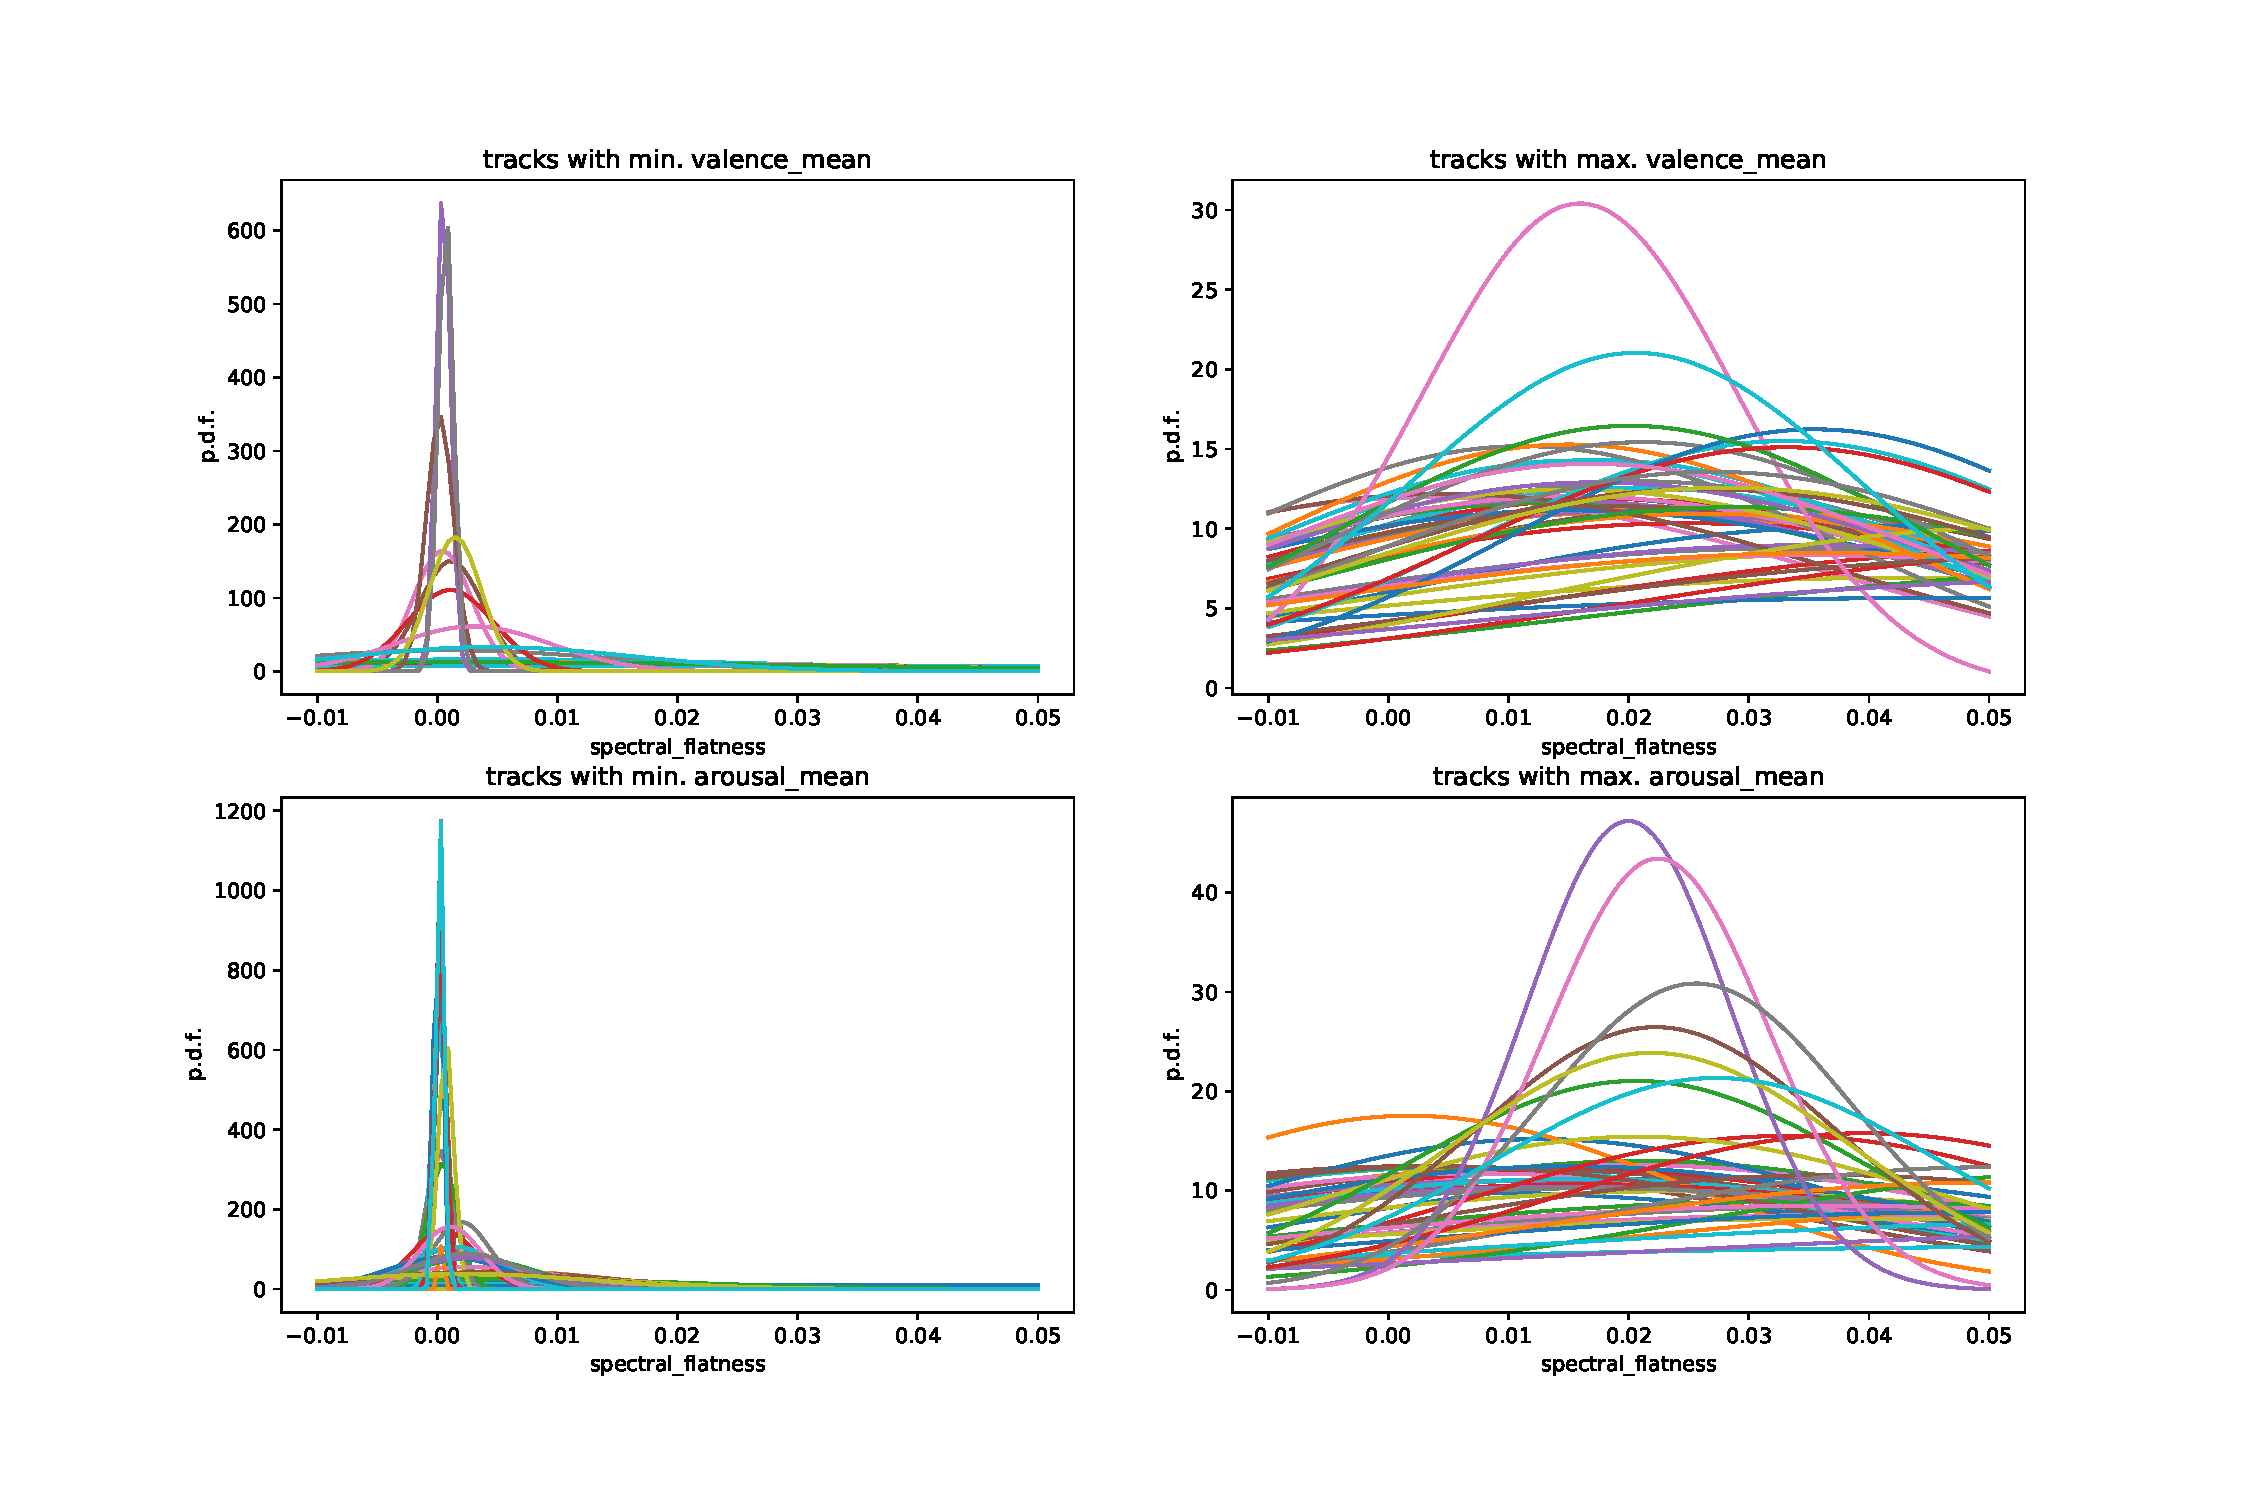
\includegraphics[width=1\linewidth]{assets/va_mean-spectral_flatness-dists.pdf}
	\caption{Spectral flatness distribution}
	\label{fig:va_mean-spectral_flatness-dists}
\end{figure}

Then, we realized that a better way to visualize features might be to plot feature-vs-annotation scatters (e.g. see figure~\ref{fig:scatter-spectral_bandwidth_amean}) and we noticed several linear relationships between a feature and valence and/or arousal values. Therefore, we used these results to make a preliminary manual feature selection. In particular we selected different features depending on the annotation to be predicted and discarded unneeded features.

\begin{figure}
	\centering
	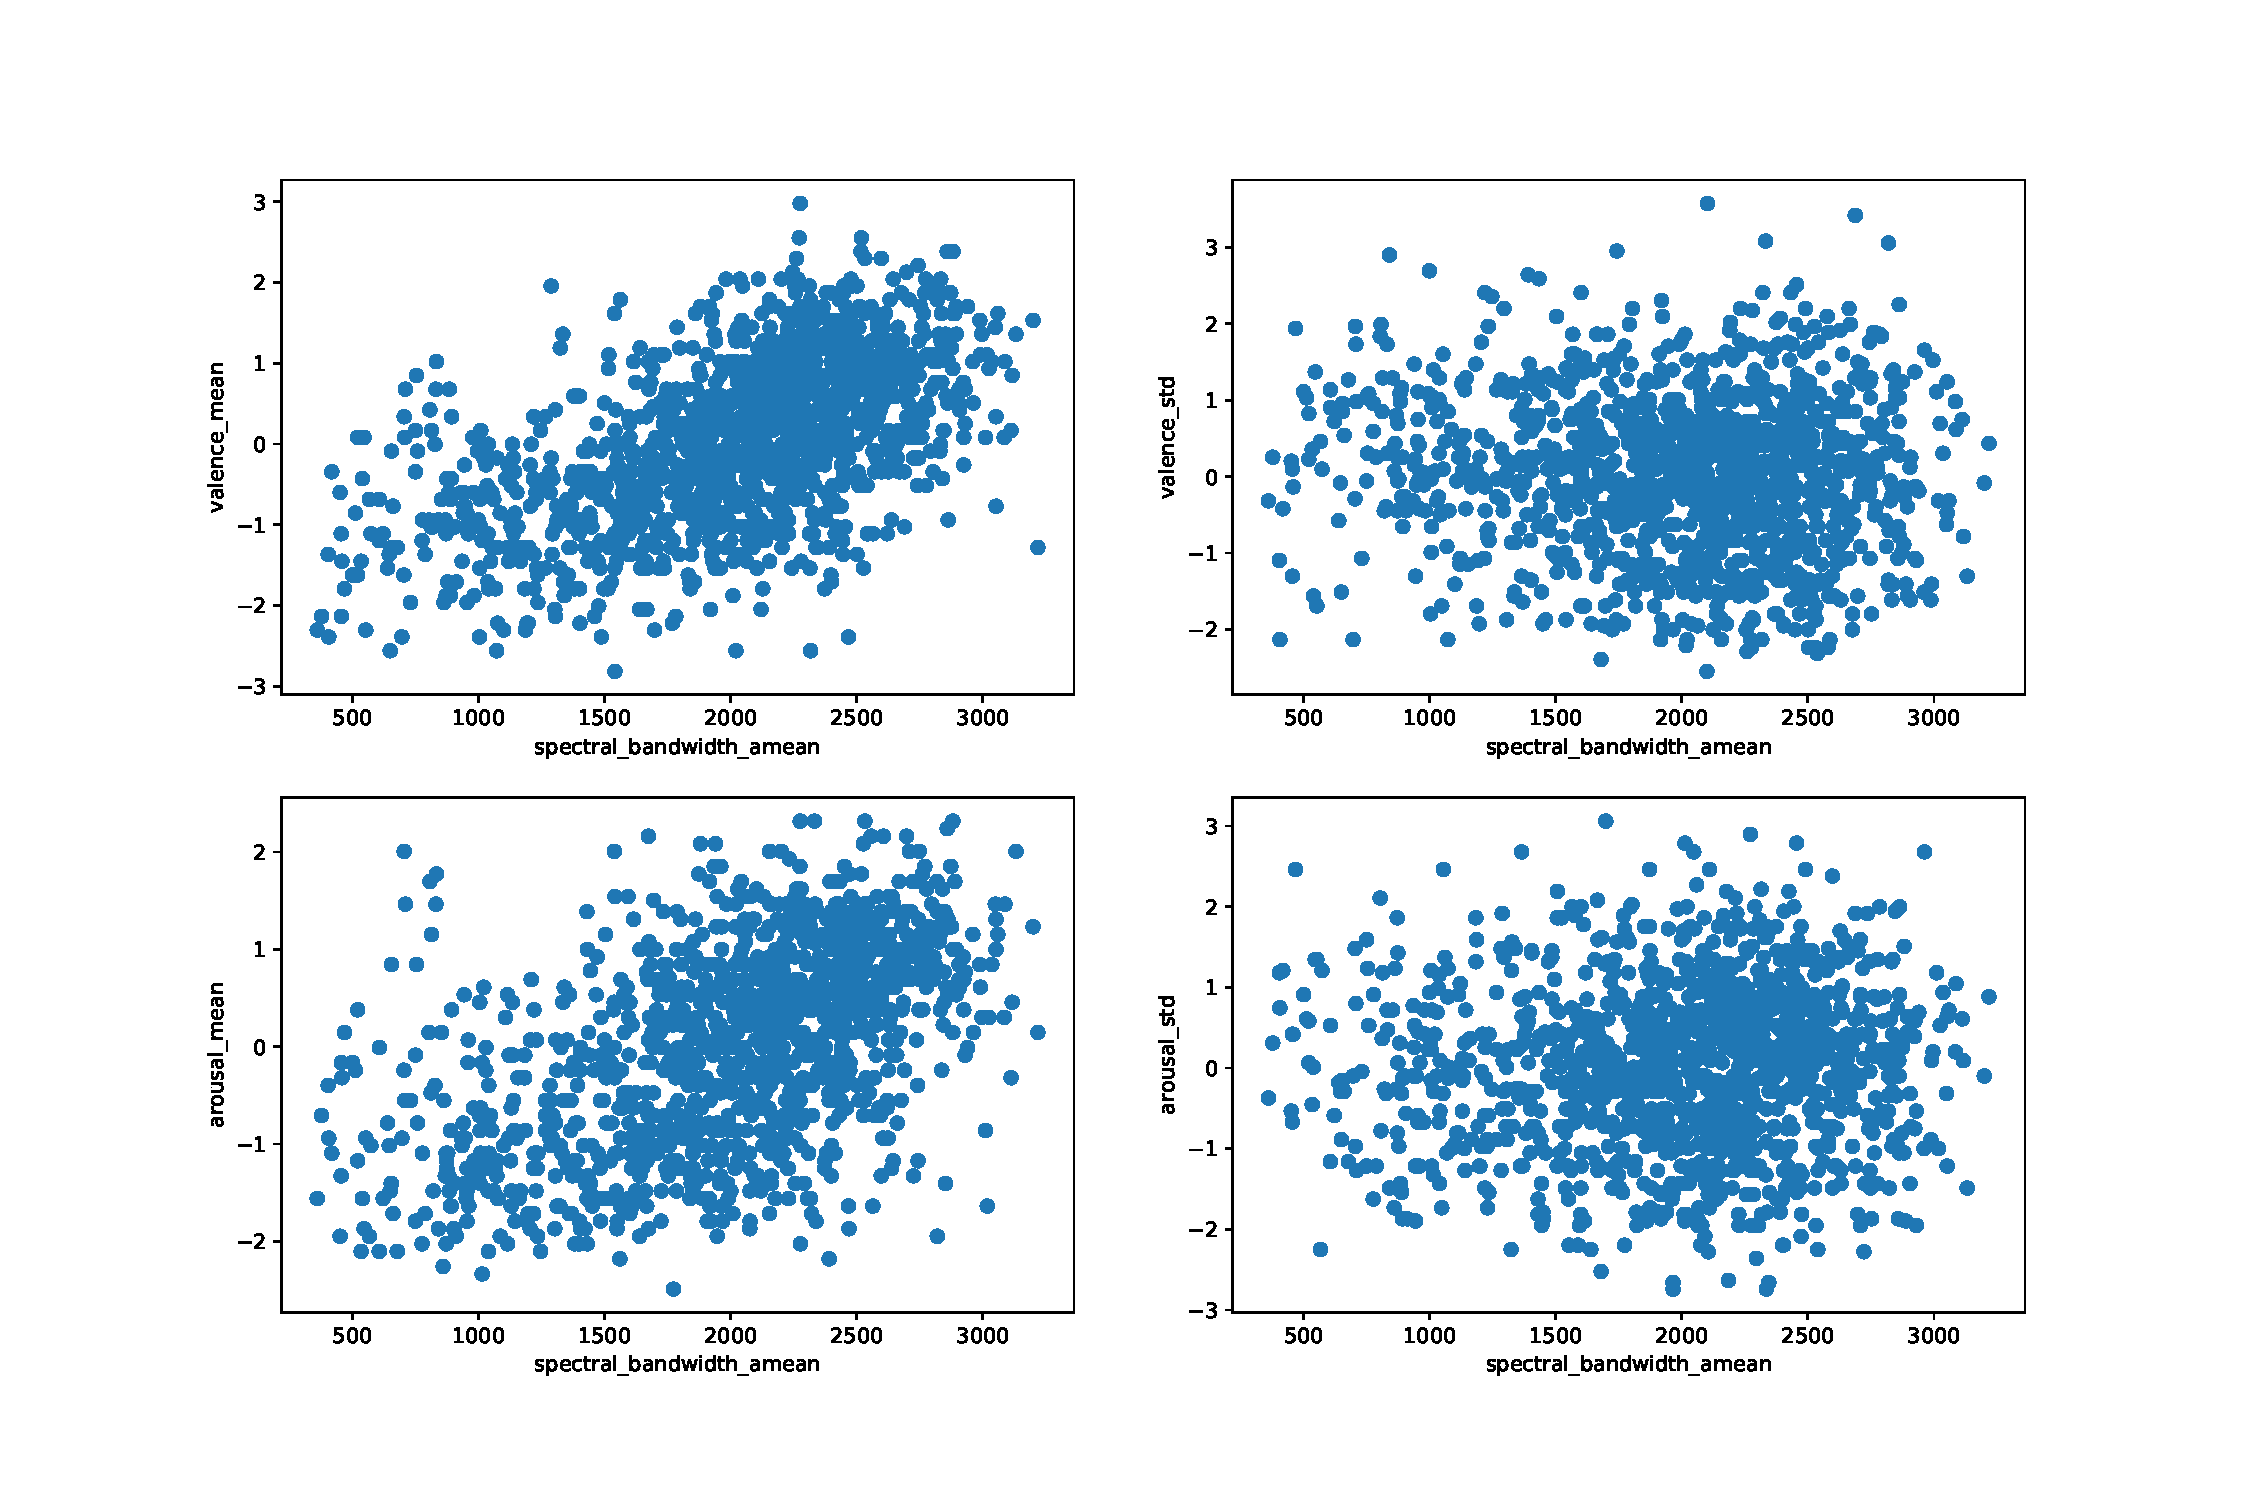
\includegraphics[width=1\linewidth]{assets/scatter-spectral_bandwidth_amean.pdf}
	\caption{Spectral Bandwidth vs. Annotations scatter plot}
	\label{fig:scatter-spectral_bandwidth_amean}
\end{figure}

Finally, in addition to manual selection, we filter out unneeded or redundant features using automatic feature selection tools, like ``recursive feature elimination'', ``select $k$-best'' and ``variance threshold''. In particular, the last two turned out to be the more effective.

For convenience, we arranged each feature processing step, including a standardization scaling (needed for some types of regressors, see section~\ref{sec:regression}), in a sklearn \texttt{Pipeline} that is executed before each fitting stage and predicting stage of the regressors. % qui una descrizione del dataset, feature e annotations
	\section{Regression models}\label{sec:regression}

Once features have been extracted, regression theory allows to predict a real value from a set of $M$ given inputs, where $M$ is the dimension of the features space.
In this context, dimensional \textbf{Music Emotion Recognition} has been considered as a regression problem where distinct regressors are trained \textit{independently} for valence and arousal. 

In particular, four regressors

\[
	r \colon \R^{M} \to \R
\]

will be trained to predict the four-element vector

\begin{center}
	[valence mean, valence std, arousal mean, arousal std]
\end{center}

Different regression models are used to find out which set of regressors best fit the data. In particular we focused on three families of regressors: \textbf{Linear Regressors}, \textbf{Support Vector Machines} and \textbf{K-Neighbors Regressors}. Performance evaluation will be achieved by means of the metrics represented by $R^2$ and $MSE$ statistics (see section~\ref{sec:metrics}).

Regressors are implemented by taking advantage of the Python library \textit{Scikit-learn}, which integrates a wide range of state-of-the-art machine learning algorithms \cite{scikit-learn}.
Regression training is not computed until the dataset is consistently rearranged and split. In fact, in order to split our collection of features and annotations in the two parts of training and testing set it will be necessary to shuffle our initial dataset so that it will be as inhomogeneous as possible in terms of music genre. \todo{ripetizione di evaluation?}
Although we will focus on Music Emotion Recognition for the global layer of the song, the regression approach is capable to fit also to music emotion variation detection (\textbf{MEVD}), considering the time evolution of features frame-by-frame for each song.

\textbf{Linear regression} is a linear model in which coefficients are computed to minimize the residual sum of squares between the observed targets in the dataset, and the targets predicted by the linear approximation \cite{scikit-learn}. 
Two other linear regressions we implemented are the \textbf{Ridge regression} with built-in cross-validation and the \textbf{Stochastic Gradient Descent regression}. 
The latter is set to be $\epsilon$-insensitive which is the same loss function used in SVR. Furthermore we provided the stopping criterion, the threshold $\epsilon$ and the $\alpha$ constant that multiplies the regularization term. The higher the value of $\alpha$, the stronger the regularization. As regards the Ridge regressor it performs a Generalized Cross-Validation, which is a form of Leave-One-Out cross-validation \cite{scikit-learn}. Out of them it turned out Ridge regressor is the most suitable algorithm for our purpose.
It represented our first attempt because of the efficiency in computational terms and consequently had the role to facilitate the search for the best features. 
Nevertheless another type of algorithm was chosen for the best regressor.

\textbf{Support Vector Regression} is our second attempt and it turned out to be the best approach.
\textbf{Support Vector Machines} represent the operation to map our features space to a higher dimensional one and learn a nonlinear function by a linear learning machine in the kernel-induced feature space, where data are more separable \cite{yang2008regression}.
The \textbf{SVR} algorithm supplied by \textit{Scikit-learn} provides an easy way to compute regressors based on different kernels and it allowed us to set the regularization parameter $C$, the tolerance for stopping criterion and the fundamental parameter $\epsilon$.
Otherwise the implementation of \textbf{NuSVR} algorithm revealed to be the most suitable. We set the parameter $\nu$ to control the number of support vectors and the penalty parameter $C$ of the error term.
Out of some attempts involving radial basis function (RBF) and sigmoid kernels we found that each of them behaves much better than Linear and K-Neighbors regressors. \todo[inline]{ricontrollare kernel (usiamo solo rbf e sigmoid), menzionare $\epsilon$ e $\nu$ e free parameters}

The latter belongs to the class of unsupervised and supervised neighbors-based learning methods.
The workflow of the \textbf{K-Neighbors regressor} is to detect the closest points in distance to the new one and extrapolate from them the value of the label.
The $k$ number of neighbors is predefined and it is up to the user. In particular, cross validation was helpful for setting the most suitable $k$ (see section~\ref{sec:cross-validation})   \todo{noi usiamo la cross per trovare $k$}
The basic implementation of the algorithm uses uniform weights for each neighbor meaning that each sample contribution is the same and it was the most efficient and suitable choice.
We also tried to assign different weights to the samples depending on the inverse of the distance from the new point.
The \texttt{KNeighborsRegressor} algorithm supplied by \textit{Scikit-learn} easily provides the keyword \texttt{weights = `distance'} to achieve this goal. \todo[inline]{in realtà con la cross quel che si comporta meglio è uniform}

Cross-validation is used to find the best parameters for each regressor and the procedure will be described in detail in the next section.
 % descrizione di metodi di regressione, selezione feature e cross-validation
	\section{Model training and evaluation}\label{sec:evaluation}

In order to avoid over-fitting and be able to evaluate our model on a real-world scenario, the dataset has to be initially shuffled (because the original dataset is ordered by genre) and split into a \emph{training set} and a \emph{testing set}.
Consequently, every kind of consideration, analysis and training was made by using the training set only, to avoid information leaking from the testing set to the training set.
A final testing can be done at the very last stage, once we are satisfied with the trained model and we are willing to test it against never seen data (see next section).

A powerful tool that can help us understand how to properly choose the features, the regressor and its parameters, and effectively evaluate the model before the final testing, is the \emph{cross-validation}, explained in the following.

\subsection{Metrics}\label{sec:metrics}

In regression theory, there are two possible metrics that can be used to assess the accuracy of a regressor, which are different from the metrics used in classification theory, since the ground truth domain is continuous.

\paragraph{Mean Squared Error}
The MSE is a measure of the expected value of the quadratic error between each predicted value $y_i$ and its true value $\hat{y}_i$, therefore a lower value indicates a better accuracy.
Given $N$ as the number of samples, it is mathematically computed as follows:

\[
	\text{MSE}(y, \hat{y}) = \frac{1}{N} \sum_{i=1}^{N} (y_i - \hat{y}_i)^2
	\qquad [0, \infty)
\]

Since it is a scale-dependent metric, it is important to contextualize it into the scale of reference (i.e. a MSE of 0.2 is worse in a domain ranging from 1 to 10 than in one ranging from 1 to 100).

\paragraph{$R^2$-score}
The coefficient of determination is a measure of how well unseen samples are likely to be predicted by the model, and it represents the ratio between the variance of the predicted values and the variance that would be predicted by the model.
Given $N$ as the number of samples, and $\bar{y}$ as the mean of the predicted values, it is mathematically computed as follows:

\[
	R^2(y, \hat{y}) = 1 - \frac{
		\sum_{i=1}^{N} (y_i - \hat{y}_i)^2
	}{
		\sum_{i=1}^{N} (y_i - \bar{y})^2
	} \qquad (-\infty, 1]
\]

It is a scale-invariant metric, therefore it is possible to compare $R^2$-scores across different domain ranges, however it is variance-dependent, so it might not be meaningful to compare it across different datasets.
A value of $1$ indicates that the regressor perfectly predicts the ground truth.
A value of $0$ indicates that the regressor always predicts the mean value $\bar{y}$, disregarding the input features.
A negative value indicates that the regressor behaves arbitrarily worse than predicting a constant.

\subsection{Cross-Validation}\label{sec:cross-validation}

It is a methodological error to evaluate metrics against the testing set and then use them to enhance the model, since this leaks information about the testing set which is supposed to be left unknown.
This phenomenon is known as \emph{over-fitting} and should be avoided.

One possible option to evaluate the model without using the testing set is to cut a separate sub-set from the training set, called \emph{validation set}, and compute the metrics against this one instead.
The drawback, however, is that this option further reduces the training set usable size.

A better approach consists in iteratively cutting a different small sub-set for validation from the training set, collect the metrics about each possible cut, and aggregate them in terms of mean and standard deviation (see figure~\ref{fig:kfolds}).
This way, the whole training set can be used.
This procedure is known as \emph{$k$-fold cross-validation}.

\begin{figure}
	\centering
	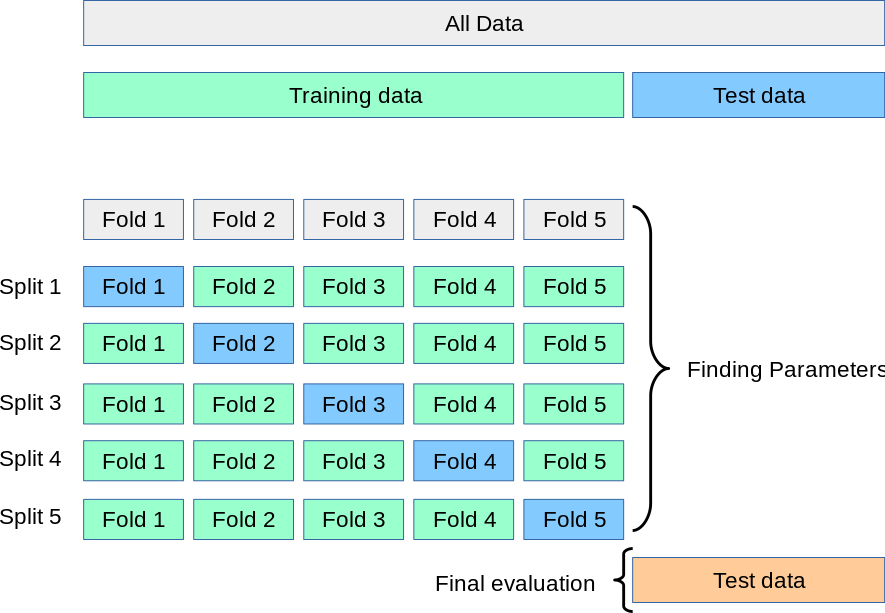
\includegraphics[width=0.6\linewidth]{assets/kfolds.png}
	\caption{$k$-fold cross-validation example with $k=5$ \cite{sklearn-crossval}}
	\label{fig:kfolds}
\end{figure}

The gathered metrics can effectively be used to evaluate the performance of the chosen regressors over the dataset.
At this point, it is possible to tune the regression model (i.e. by changing the free parameters of the regressors) without the risk of over-fitting (see figure~\ref{fig:grid-search-workflow}).

\begin{figure}
	\centering
	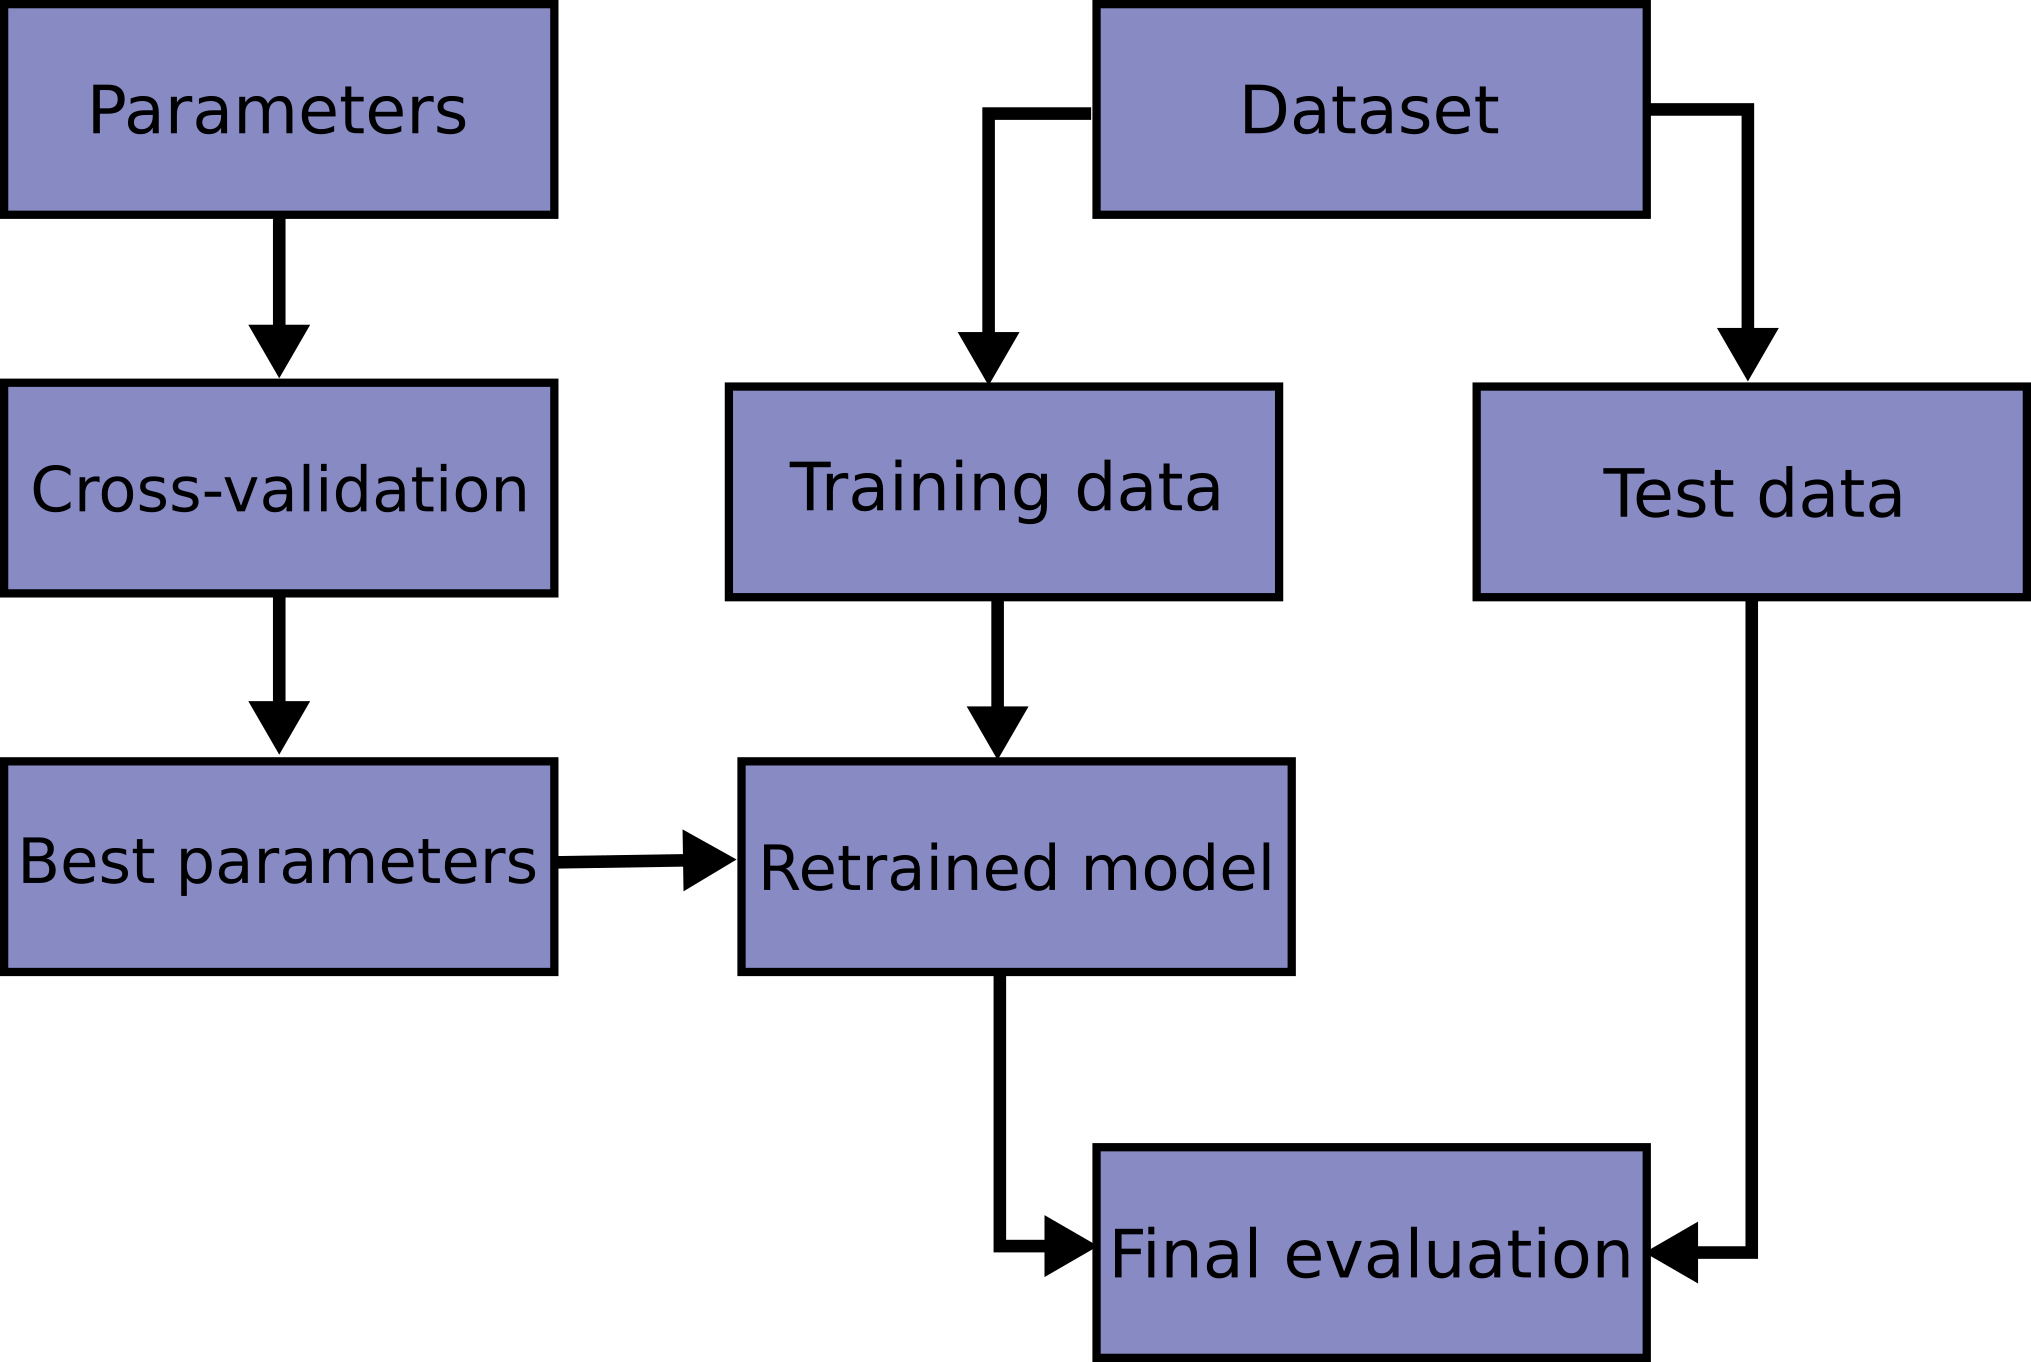
\includegraphics[width=0.5\linewidth]{assets/grid_search_workflow.png}
	\caption{Grid Search Workflow \cite{sklearn-crossval}}
	\label{fig:grid-search-workflow}
\end{figure}


\subsection{Enhancing the model}\label{sec:enhance-model}

The sklearn library provides a function \texttt{GridSearchCV()} for automatically selecting the best parameters for a given estimator, based on a grid of possible combinations.

At first, we computed the scores over a simple \texttt{LinearRegression} to evaluate the feature selection stage (see section~\ref{sec:features}).
Then we took advantage of the grid search to first optimize the linear model by using a Stochastic Gradient Descent regressor and a Ridge regressor with integrated cross-validation optimization.
We finally used again the grid search to find the suitable parameters (see section~\ref{sec:regression}) for $\nu$-SVM, $\epsilon$-SVM and KN-regressor.
For example, the best parameters found for the $\nu$-SVM regressor are reported in tables~\ref{table:cross-params-svr}.

\begin{table}
	\centering
	\begin{tabular}{lccc}
		\toprule
		& kernel & $C$ & $\nu$ \\
		\midrule
		valence mean & rbf & $10$ & $0.75$ \\
		valence std & rbf & $0.1$ & $0.25$ \\
		arousal mean & rbf & $1$ & $0.5$ \\
		arousal std & rbf & $0.1$ & $0.75$ \\
		\bottomrule
	\end{tabular}
	\caption{Best parameters for $\nu$-SVM regressor}
	\label{table:cross-params-svr}
\end{table}

%\begin{table}
%	\centering
%	\begin{tabular}{lcccc}
%		\toprule
%		& loss function & $\alpha$ & $\epsilon$ & tolerance \\
%		\midrule
%		valence mean & $\epsilon$-insensitive & $10^{-3}$ & $10^{-3}$ & $10^{-4}$ \\
%		valence std & $\epsilon$-insensitive & $10^{-2}$ & $10^{-2}$ & $10^{-4}$ \\
%		arousal mean & $\epsilon$-insensitive & $10^{-2}$ & $10^{-3}$ & $10^{-3}$ \\
%		arousal std & $\epsilon$-insensitive & $10^{-3}$ & $10^{-1}$ & $10^{-4}$ \\
%		\bottomrule
%	\end{tabular}
%	\caption{Best parameters for SGD regressor}
%	\label{table:cross-params-sgd}
%\end{table}

After refining the feature selection, we extracted the metrics of the best found estimators (see table~\ref{table:cross-scores}). It can be observed that, even after several attempts of feature selection (both manual and automatic), and optimization through cross-validation, no regressor could obtain a significant positive $R^2$-score for the values of ``valence std'' and ``arousal std'', and the obtained $R^2$-scores for ``valence mean'' and ``arousal mean'' were still quite low. This might be a consequence of the poor quality of the provided dataset, which required some preprocessing step on it that we didn't manage to accomplish.

\begin{table}
	\centering
	\begin{tabular}{lcccc}
		\toprule
		& valence mean & valence std & arousal mean & arousal std \\
		\midrule

		Linear & 0.44 ± 0.19 & -0.10 ± 0.12 & 0.39 ± 0.13 & -0.13 ± 0.18 \\
		SGD & 0.41 ± 0.25 & -0.11 ± 0.14 & 0.36 ± 0.19 & -0.16 ± 0.20 \\
		Ridge & 0.46 ± 0.16 & -0.04 ± 0.09 & 0.41 ± 0.14 & -0.10 ± 0.16 \\

		$\nu$-SVM & 0.40 ± 0.18 & 0.01 ± 0.06 & 0.48 ± 0.16 & 0.01 ± 0.07 \\
		$\epsilon$-SVM & 0.42 ± 0.18 & 0.02 ± 0.05 & 0.41 ± 0.13 & 0.01 ± 0.07 \\

		K-neighbors & 0.40 ± 0.08 & -0.06 ± 0.09 & 0.40 ± 0.16 & -0.07 ± 0.10 \\
		\bottomrule
	\end{tabular}
	\caption{Cross-validation $R^2$-scores with 95\,\% confidence intervals}
	\label{table:cross-scores}
\end{table}

However, a meaningful evaluation of the trained model can be still obtained by comparing the scores of the cross-validation against the scores obtained by the final testing stage.
This way, we can assess how worse the model will behave when we input never seen data (see section~\ref{sec:conclusions}).
In particular, given the results in table~\ref{table:cross-scores}, we decided to use Ridge, $\nu$-SVM and KN-regression as candidates for the final testing stage, as they seemed to be the best scoring regressors for each family of regression models considered.
 % estrazione di metriche e valutazioni
	\section{Final testing and conclusions}\label{sec:conclusions}

Once we refined our model at the best could, we evaluated it against never seen data, by comparing the values predicted by the model, when the testing set is provided as input, against the true values of the annotations in the testing set. As already mentioned in section~\ref{sec:cross-validation}, once the final testing is done, we avoided going back to the model and make further tweaks, as this would have led to over-fitting.

For the final test we used the metrics of MSE and $R^2$-score (see section~\ref{sec:metrics}) and obtained the values reported in table~\ref{table:eval-metrics}. Despite several attempts and tests with different combinations of features, our results are not still optimal, in particular the $R^2$-score associated to the regressors of the two standard deviations. \todo[inline]{è una ripetizione della fine di evaluation, quel che conta è confrontare gli R2 di cross con R2 finali}

We also extracted scatter plots comparing the predictions of each regressor against the true values of the testing set. In  figure~\ref{fig:eval-scatter} is depicted the case of $\nu$-SVM, which turned out to be the best model fitting the data. In the best case scenario, these scatters should draw a 45° line. In our case, the scattering of ``valence std'' and ``arousal std'' clearly outline the bad $R^2$-scores obtained for these annotations. \todo{da finire}

The motivation of our results could be related to the composition of the dataset and the fact that we used only the part containing static annotations. A dynamic approach in which we consider values related to temporal windows and not to the total length of the music piece could have given different results. \todo{riscriverlo meglio forse}


\begin{table}
	\centering
	\subcaptionbox{MSEs}{
		\begin{tabular}{lcccc}
			\toprule
			& valence mean & valence std & arousal mean & arousal std \\
			\midrule
			Ridge & 0.53 & 1.09 & 0.54 & 1.18 \\
			$\nu$-SVM & 0.58 & 1.00 & 0.49 & 1.09 \\
			K-neighbors & 0.62 & 1.00 & 0.61 & 1.08 \\
			\bottomrule
		\end{tabular}
	}
	\subcaptionbox{$R^2$-scores}{
		\begin{tabular}{lcccc}
			\toprule
			& valence mean & valence std & arousal mean & arousal std \\
			\midrule
			Ridge & 0.45 & -0.08 & 0.45 & -0.09 \\
			$\nu$-SVM & 0.40 & 0.01 & 0.50 & 0.00 \\
			K-neighbors & 0.35 & 0.01 & 0.39 & 0.00 \\
			\bottomrule
		\end{tabular}
	}
	\caption{Final evaluation metrics}
	\label{table:eval-metrics}
\end{table}

\begin{figure}
	\centering
	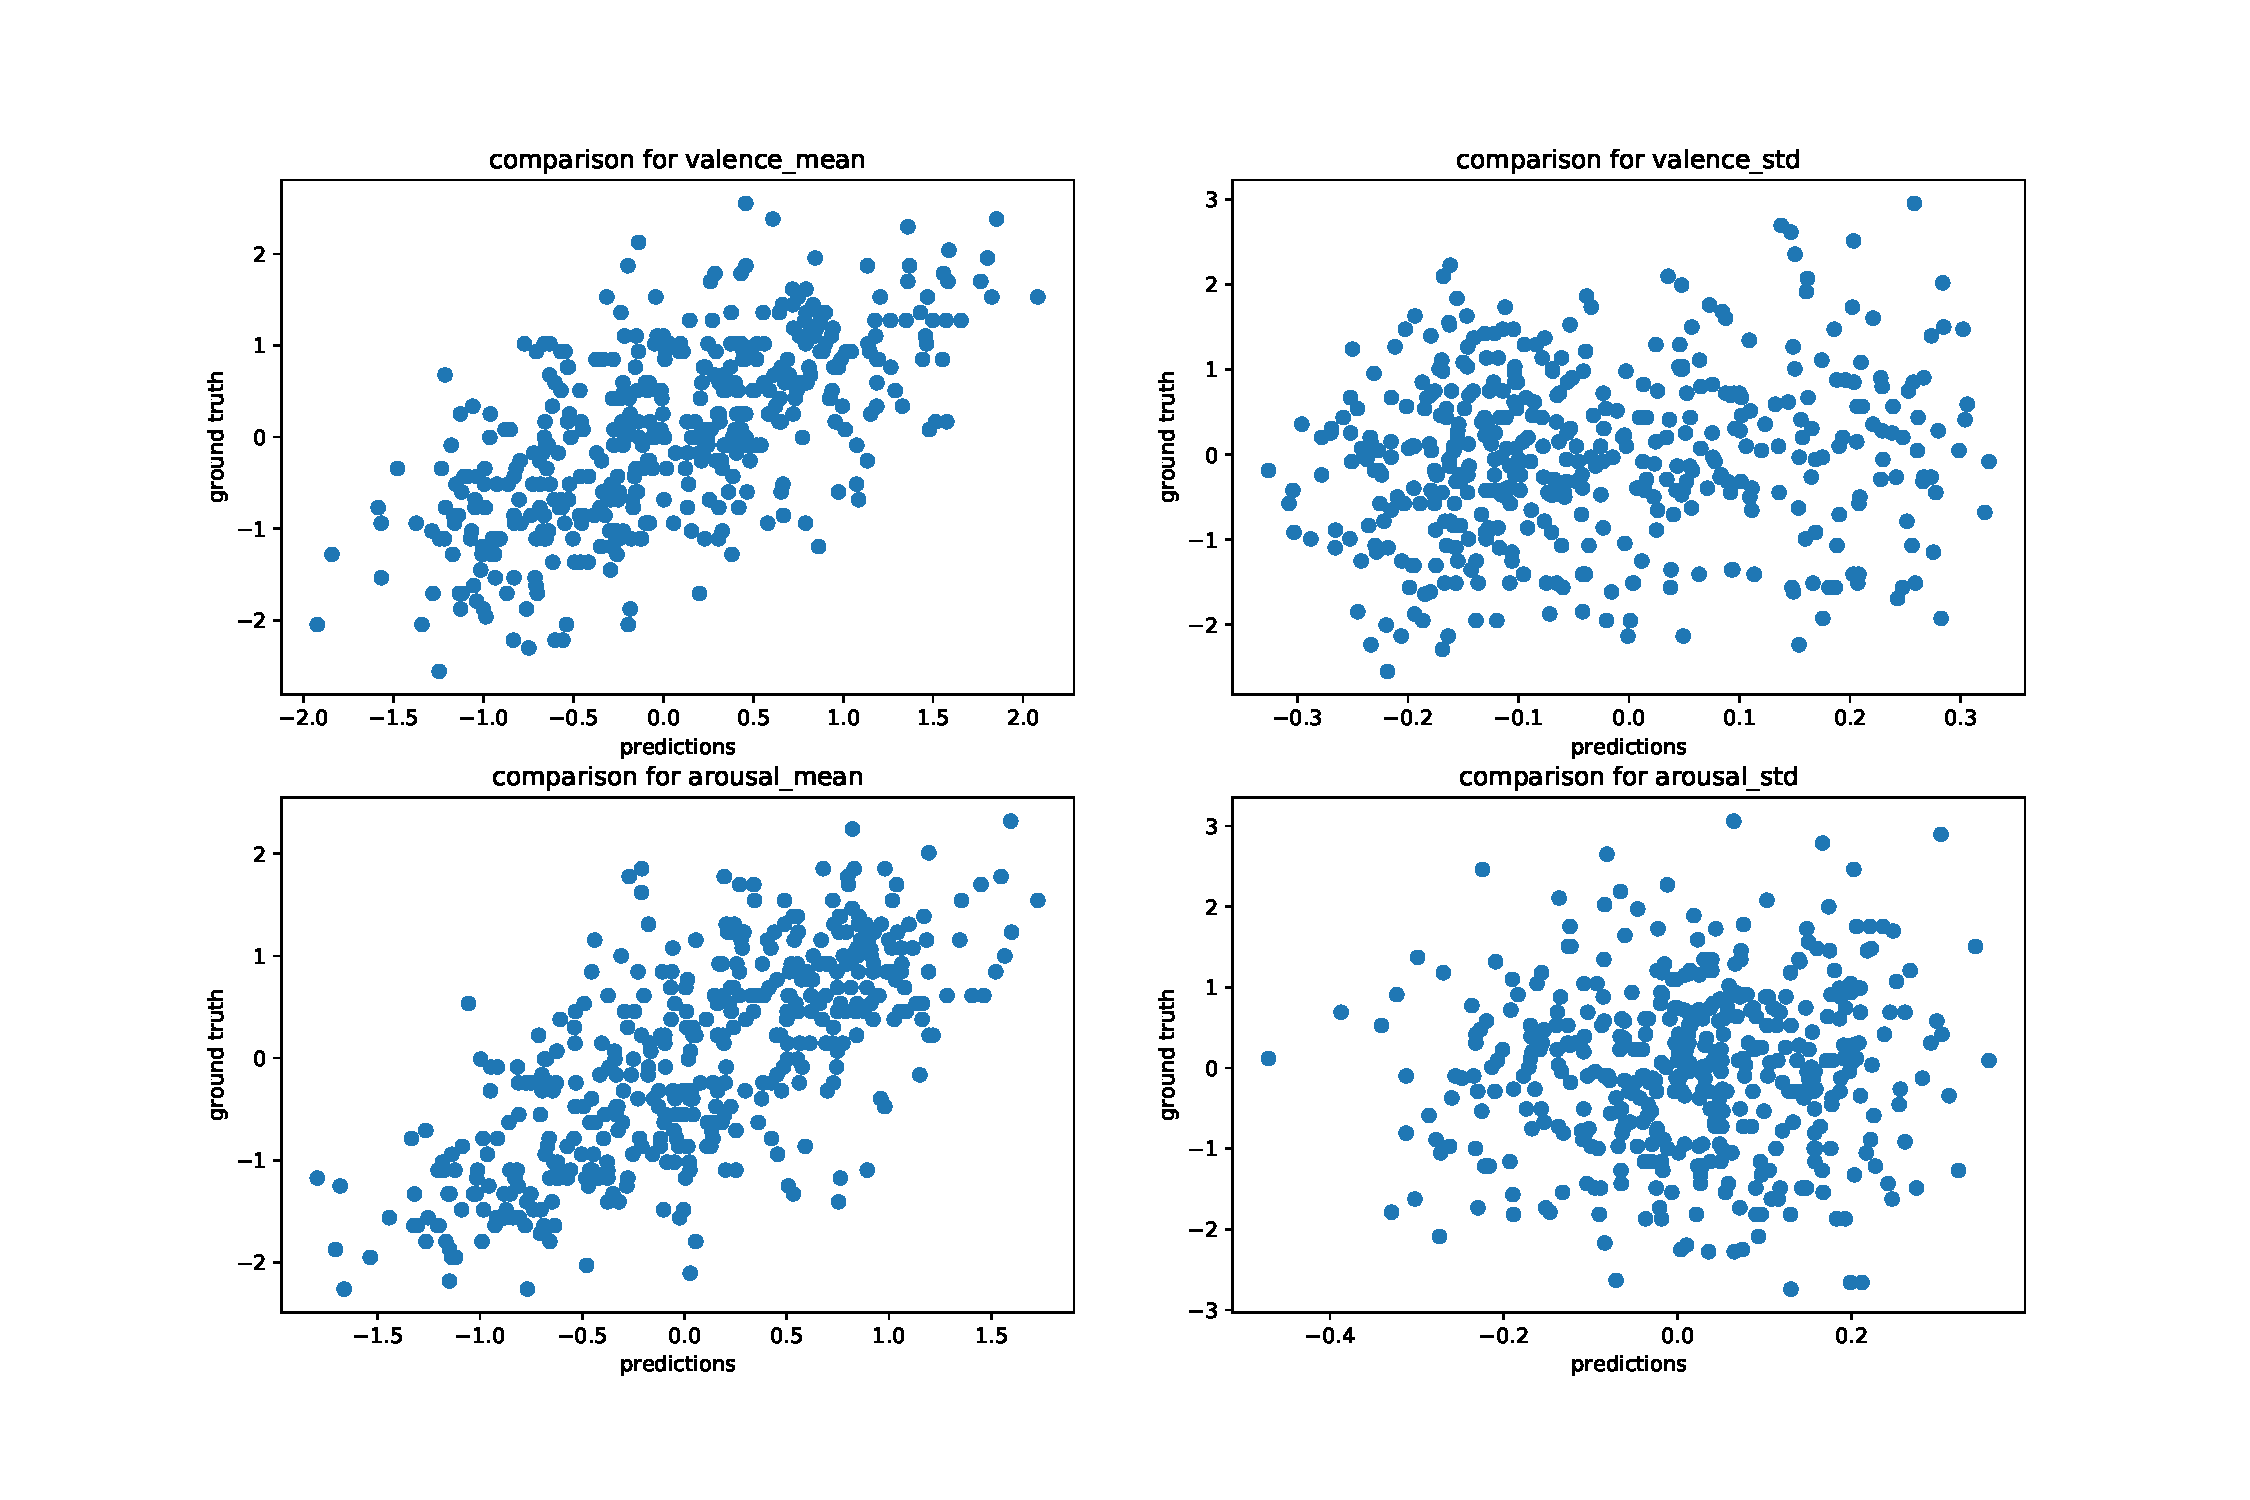
\includegraphics[width=\linewidth]{assets/predictions-scatter.pdf}
	\caption{predictions vs. ground-truth scatter for SVM regression}
	\label{fig:eval-scatter}
\end{figure}


 % conclusioni e sviluppi futuri

	\bibliographystyle{plain}
	\bibliography{bibliography}

\end{document}
